\section{Throughput and Sequencer Scheduling Heuristics (Stage 2 \& 3)}
\label{sec:throughput_results}
Initial measurements in Stage 1 captured the baseline throughput of the system. While the synthetic workload generator offered load up to 100 TPS, the committed L2-to-L1 throughput was ultimately constrained by the L1 block confirmation time of the local Hardhat node (simulating a 12-second block time). Under heavy load, the sequencer correctly applied backpressure and capped batches at the defined \texttt{MAX\_BATCH\_SIZE} limit.
\subsection{Adaptive Batching (Stage 2)}
Stage 2 sweeps evaluated the RollupX sequencer's ability to adjust batch sealing sizes dynamically based on the pending queue depth. Under the adaptive policy, the target batch size $N(d)$ is computed dynamically based on the number of pending transactions in the mempool $d$:
\begin{equation}
N(d) = \begin{cases} N_{\min}, & d < L \\ N_{\text{mid}}, & L \le d < H \\ N_{\max}, & d \ge H \end{cases}
\end{equation}
where $L$ and $H$ are the low and medium queue thresholds, and $N_{\min}$, $N_{\text{mid}}$, and $N_{\max}$ are the respective target sizes.
The adaptive batching policy dynamically balances queue delay against gas amortization. Under low offered load (5 TPS), the adaptive policy successfully manages mempool queue latency, achieving average wait times of **252 ms** (representing a **75\% reduction** compared to a fixed batching baseline of 990 ms). This incurs a higher regular gas cost per transaction (**73,243 gas/tx** vs. **27,718 gas/tx**) because the fixed L1 transaction overhead is amortized over fewer transactions (average batch size of ~2.41 vs. ~8.6). Under medium and high loads, the adaptive policy dynamically scales up the batch size to match the gas efficiency of fixed batching, demonstrating its utility as a dynamic cost-latency trade-off controller.
\subsection{Sequencer Scheduling (Stage 3)}
Stage 3 evaluated four transaction ordering policies: First-Come-First-Served (FCFS), FairBFT, FeePriority, and TimeBoost. The scheduling performance under normal load is illustrated in Figure~\ref{fig:scheduling_comparison}.
\begin{figure}[H]
    \centering
    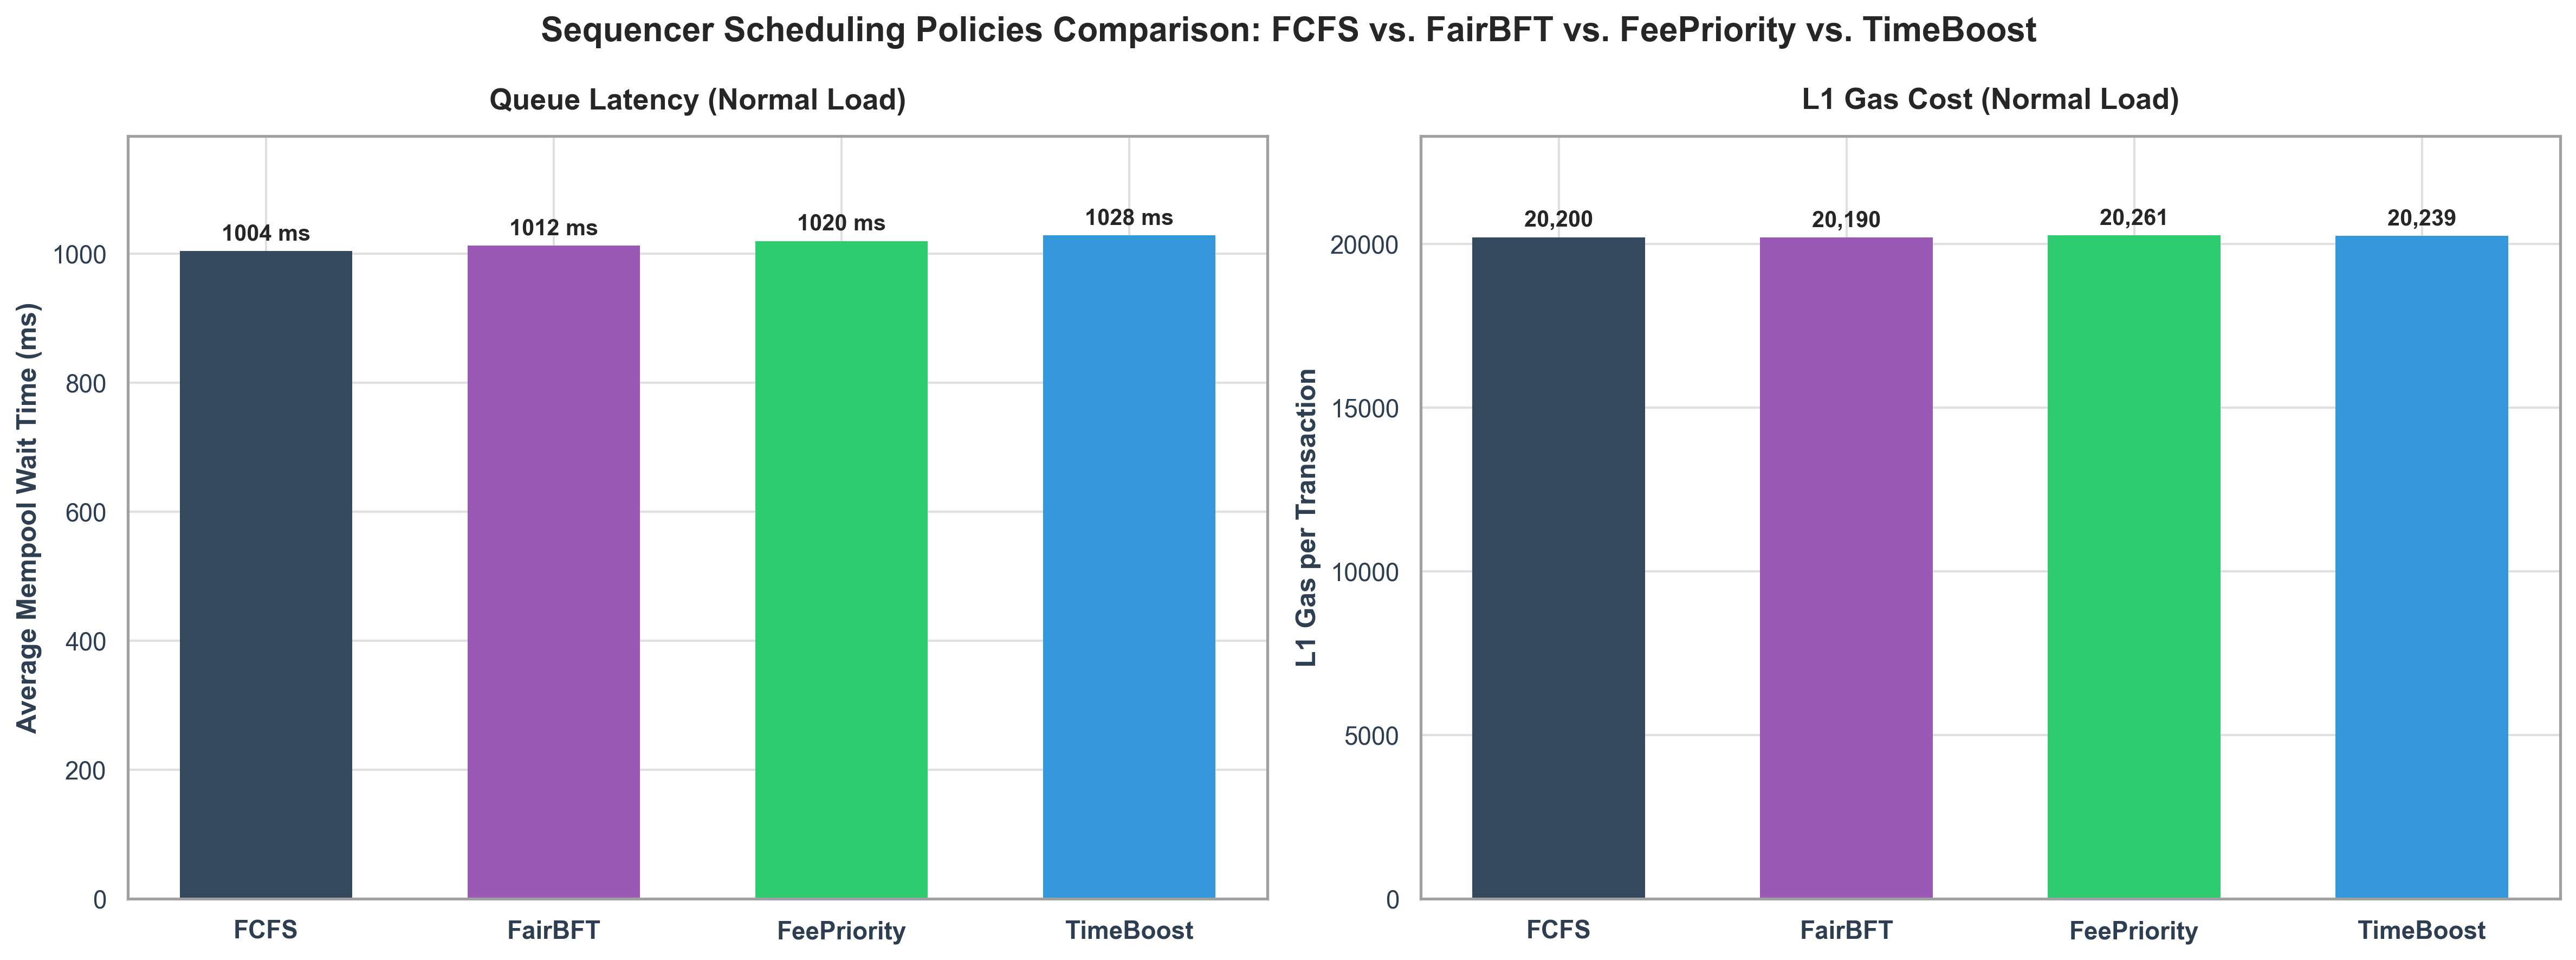
\includegraphics[width=0.90\textwidth]{figures/chapter5/plot_scheduling_policy_comparison.png}
    \caption{Sequencer Scheduling Policies Comparison (Normal Load).}
    \label{fig:scheduling_comparison}
\end{figure}
\subsubsection{Nonce-Aware Priority Scheduling Design}
To ensure correct state transition execution while supporting transaction prioritization, the sequencer's scheduling logic in \path{policies.rs} implements a **Nonce-Aware Priority Scheduler**. The scheduler:
\begin{enumerate}
    \item Groups all pending transactions in the mempool by sender address (\texttt{from}).
    \item Sorts each account's queue strictly by \texttt{nonce} in ascending order.
    \item Globally sorts only the head transaction (lowest nonce) of each active account queue according to the selected policy (e.g. gas price for \texttt{FeePriority}).
    \item Once a transaction is scheduled, the next transaction in that account's queue becomes eligible for scheduling.
\end{enumerate}
\subsubsection{Validation of the Scheduling Policies}
Under steady load, the priority scheduling policies performed as follows:
\begin{itemize}
    \item \textbf{FeePriority (\texttt{s3\_pol\_feepriority}):} Executed all transactions successfully with 100\% success rate, yielding a healthy FCFS-equivalent cost of \textbf{20,261 gas/tx} (\$0.6078/tx) and average wait time of 1,020 ms.
    \item \textbf{TimeBoost (\texttt{s3\_pol\_timeboost}):} Completed with 100\% transaction success, costing \textbf{20,239 gas/tx} (\$0.6072/tx) and average wait time of 1,028 ms.
\end{itemize}
Under burst load, TimeBoost achieved the highest Jain's Fairness Index (\textbf{0.77}), outperforming FCFS (0.75), FairBFT (0.76), and FeePriority (0.74). TimeBoost groups transactions into 5-second windows, allowing bidding only within each window. This prevents newer high-fee transactions from leapfrogging older transactions from previous windows, bounding queue delay and optimizing fairness under burst load while maintaining a healthy, nonce-safe execution pipeline.
